\documentclass[12pt, letterpaper]{article}
\usepackage{graphicx}
\usepackage[utf8]{inputenc}
\usepackage[english]{babel}
\usepackage{biblatex}
\addbibresource{mybibliography.bib}

\title{Course Project - Pymagicc}
\author{Ehsan Rafiei Azad}
\date{June 20, 2021}

\begin{document}

\maketitle

\section{Introduction}
Pymagicc\footnote{https://pymagicc.readthedocs.io/en/latest/index.html} is a Python wrapper around the reduced complexity climate model MAGICC6\footnote{http://magicc.org/}.  
 MAGICC  (Model  for  the  Assessment  of  Greenhouse  Gas  In-duced Climate Change) is widely used in climate policy analyses to assess future emissions pathways,  such as in the Intergovernmental Panel on Cli-mate Change’s Fifth Assessment Report, or to model the physical aspects of climate change in Integrated Assessment Models (IAMs).  Pymagicc makes it simple to deploy and then use the MAGICC model from Python and modify all MAGICC model parameters and emissions scenarios directly from Python.It may be used in climate research for various purposes, including mitigation scenario analysis, Integrated Assessment Models, complicated climate model emulation, uncertainty assessments, and climate science education and communication.For this project,  I tried to have some analysis and visualizations based on the predefined RCP datasets. I  have  three  tasks,  and  all  of  them  are according to the examples in the official documentation.
 
For this project,  I tried to have some analysis and visualizations based on the predefined  RCP  datasets.   I  have  three  tasks,  and  all  of  them  are according to the examples in the official documentation.I also used the Matplotlib library for my visualization part.

\section{Tasks}

Climate scientists\cite{o2017roads} believe that our planet will continue to warm for the rest of this century and beyond. Carbon dioxide and other heat-trapping "greenhouse" gases produced by human activities are the primary cause of this rise.
So, here in this project, I decided to show the amount of CO2 in the atmosphere and its impact on global warming with two following graphs.

\subsection{Concentration to emissions by CO2}
The first task is representing the concentration of CO2 in the atmosphere and the rate of its emissions. As you can see, now we are almost at the highest level of pollution.

\begin{figure}[hbt!]
\centering
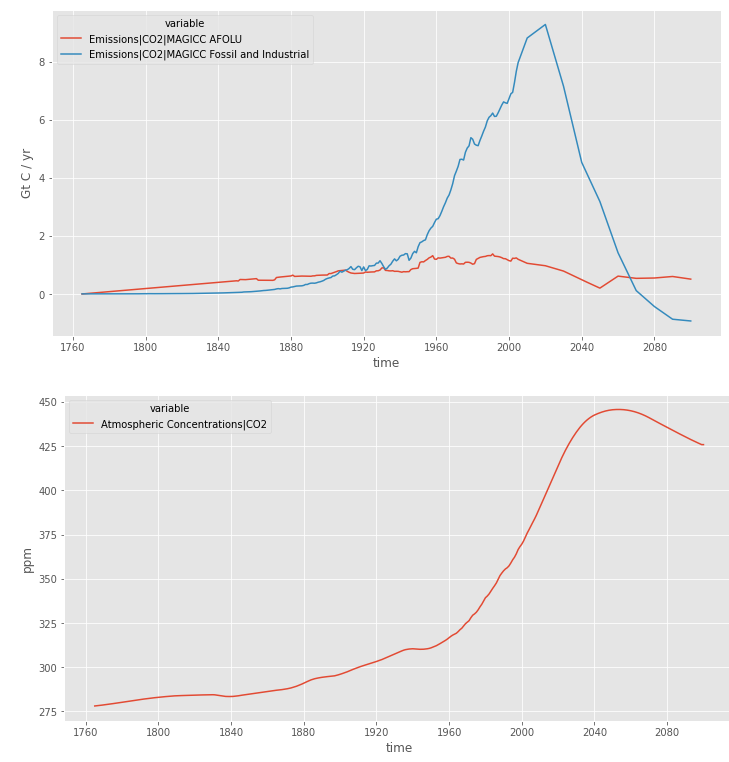
\includegraphics[scale=0.7]{Task1.PNG}
\caption{Concentration to emissions by CO2}
\label{fig:Task1}
\end{figure}

\subsection{Global Mean Temperature Projection}
In the second task, I demonstrated a graph of global temperature from 1850 to 2100. Based on this visualization, we can forecast the global mean temperature until the end of the century.

\begin{figure}[hbt!]
\centering
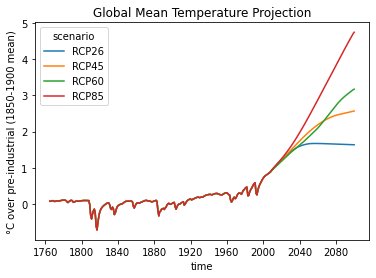
\includegraphics[scale=0.7]{Task2.PNG}
\caption{Global Mean Temperature Projection}
\label{fig:Task2}
\end{figure}

\section{Conclusions}
Now I can say that I attempted to learn how to use a new python library, like Pymagicc, to make meaningful charts, and the result of this project shows that the increase in the level of CO2 will cause global warming subsequently. 

\printbibliography
\end{document}
